\documentclass[tikz,border=2pt]{standalone}
\usepackage{amsmath}
\usetikzlibrary{arrows.meta}
\begin{document}
% Chicken (table on the page): p = P(player 1 plays T), q = P(player 2 plays T). BR_1 is T for q<1/3,
% S for q>1/3; BR_2 likewise in p. They meet at (1,0)=(T,S), (0,1)=(S,T) and (1/3,1/3).
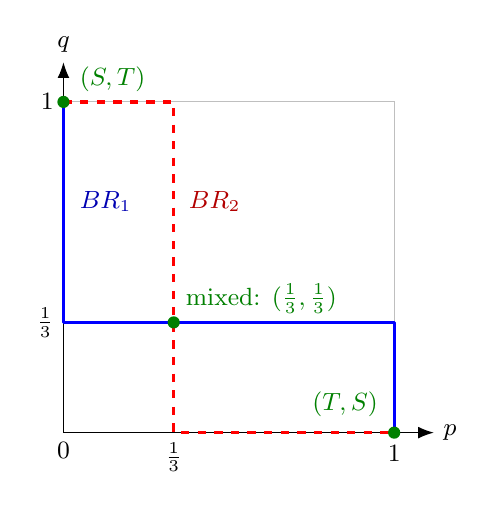
\begin{tikzpicture}[font=\small, >={Latex[length=2mm]}, x=4.2cm, y=4.2cm]
  \draw[gray!50, thin] (0,0) rectangle (1,1);
  \draw[->] (0,0) -- (1.12,0) node[anchor=west] {$p$};
  \draw[->] (0,0) -- (0,1.12) node[anchor=south] {$q$};
  \node[anchor=north] at (0,0) {$0$};
  \node[anchor=north] at (1/3,0) {$\tfrac13$};
  \node[anchor=north] at (1,-0.01) {$1$};
  \node[anchor=east] at (0,1/3) {$\tfrac13$};
  \node[anchor=east] at (0,1) {$1$};
  % BR_1 (blue): p=1 for q<1/3, any p at q=1/3, p=0 for q>1/3
  \draw[blue, very thick, line join=round] (1,0) -- (1,1/3) -- (0,1/3) -- (0,1);
  % BR_2 (red, dashed): q=1 for p<1/3, any q at p=1/3, q=0 for p>1/3
  \draw[red, very thick, dashed, line join=round] (0,1) -- (1/3,1) -- (1/3,0) -- (1,0);
  \node[blue!70!black, anchor=west] at (0.02,0.7) {$BR_1$};
  \node[red!70!black, anchor=west] at (0.35,0.7) {$BR_2$};
  % equilibria
  \foreach \x/\y in {0/1, 1/0, 0.3333/0.3333} \fill[green!50!black] (\x,\y) circle (2.2pt);
  \node[green!50!black, anchor=south west] at (0.02,1.0) {$(S,T)$};
  \node[green!50!black, anchor=south east] at (0.98,0.02) {$(T,S)$};
  \node[green!50!black, anchor=south west, fill=white, inner sep=1pt] at (0.36,0.35) {mixed: $(\tfrac13,\tfrac13)$};
\end{tikzpicture}
\end{document}
